\section{Introduction}

In recent years, the world is becoming more virtual than we ever thought it would be. Many video service providers, such as YouTube, roll out Virtual Reality (VR) videos which provide immersive experience to users. While consuming VR videos, users can change their viewpoint, resulting in an interactive experience than consuming traditional videos with a fixed viewing direction. However, VR videos' high demand of resolution and bitrates hinder their wide spread over the Internet. How to provide high user-perceived quality with limited bandwidth becomes the biggest problem in VR video streaming.

Viewpoint-adaptive streaming is regarded as a promising way to solve the problem. It assumes that a object's user-perceived quality depends on the distance from it to user's viewpoint\cite{distance}. It allocates high bit-rate for objects near user's viewport, and allocates low bit-rate for objects far from user's viewport. 

However, viewpoint-adaptive streaming is a very coarse approximation of user-perceived quality, since user-perceived quality is not only related to object-viewpoint distance. Many prior works state that it is related to some human visual characteristics, such as luminance\cite{PSPNR}, \cite{luminance1}, texture complexity\cite{PSPNR}. We model these visual characteristics into our potential improvement evaluation, and result shows that we can save 30\% bandwidth without decrease of user perceived quality. Moreover, our user study shows that in VR video display, user-perceived quality is also related to viewpoint moving speed and Depth-of-Field (DoF). When we take consideration of these visual characteristics, we can further save 20\% bandwidth without decrease of user perceived quality.

Although these insights about user-perceived quality give us promising potential improvement, optimizing perceived quality in real VR streaming system is challenging in three aspects:

\begin{itemize}

\item \textbf{Challenge 1: Traditional Human Visual System (HVS) models can not measure perceived quality in VR video display.} Perceived quality can be well-measured in traditional video display by modeling human visual system. However, perceived quality in VR display is very different from traditional video display. So current models can not be applied. We need to build a new model to quantify perceived quality in VR display.

\item \textbf{Challenge 2: Traditional grid-like video tiling scheme performs poorly in perceived quality optimization.} To allocate different bitrate to different objects, we need to cut the video into several spatial tiles which can be independently encoded / decoded. In traditional grid-like tiling scheme, videos are cut into m*n rectangular tiles of equal size. However, in a coarse-grained tiling, performance of quality allocation is poor. In a fine-grained tiling, serious bitrate efficiency problem occurs in video encoding. Both of them make the performance of perceived quality optimization far from the optimal value.

\item \textbf{Challenge 3: Information needed for perceived quality computation is disparted on server-side and client-side.} Perceived quality depends on both video content and user behavior, so it can not be pre-computed as some traditional quality metrics (such as PSNR, MSE, SSE). Client needs to compute the perceived quality of each bitrate allocation and then make decision in realtime. However, to get information of video content with current DASH, client has to pre-request the information of each pixel from server. This communication overload even exceed the overload of actual video streaming.

\end{itemize}

In this work, we address technical challenges above, then present the design and implementation of Perceived Quality driven VR Streaming (PQVRS). PQVRS is built on three key insights:

\begin{itemize}

\item \emph{Perceived quality model in VR display can be built by simply adding several new factors on traditional perceived quality model.} Although there are several new factors which influence perceived quality in VR display, and the correlation between them may be complex, we find that their influence to perceived quality can be considered independently. So we only need to measure the perceived quality due to each of new insights, and then add them to current perceived quality model.

\item \emph{Video tiling strategy can be optimized on server side.} Since traditional grid-like tiling method fail to exactly catch objects in videos, it limits the performance of perceived quality driven rate allocation. Tiling video by objects can solve this problem. Moreover, information of objects is only related to videos, object-based tiling can be completed in advance on server-side.

\item \emph{Perceived quality computation can be decoupled.} Although server has no information about user behavior, it can still compute perceived quality with each possible user behavior situations offline. Then server sends the results to client, client combine the computation result and actual user behavior to obtain final perceived quality.

\end{itemize}

Although accurately computing perceived quality needs the value of each pixel of each frame, it can be well-approximated on client-side using much less information.

Taken together, these insights enable us to engineer a Perceived Quality driven VR Streaming (PQVRS). In PQVRS, we decouple the visual characteristics due to video objects and user viewpoint, and build the VR streaming system which consider visual characteristics of video objects completely on server-side, and considers visual characteristics of user viewpoint pattern completely on client-side.

We implemented a prototype of PQVRS. We ran a pilot study on one content provider with x sessions. Our experiments show that PQVRS can save 45\% bandwidth compared with state-of-art VR streaming solutions, without decrease of perceived quality. In real-world adaptive streaming with unstable throughput, we obtain significantly higher user-perceived quality without introducing stalling. (Fig. \ref{first_image})

    \begin{figure}
  \centering
  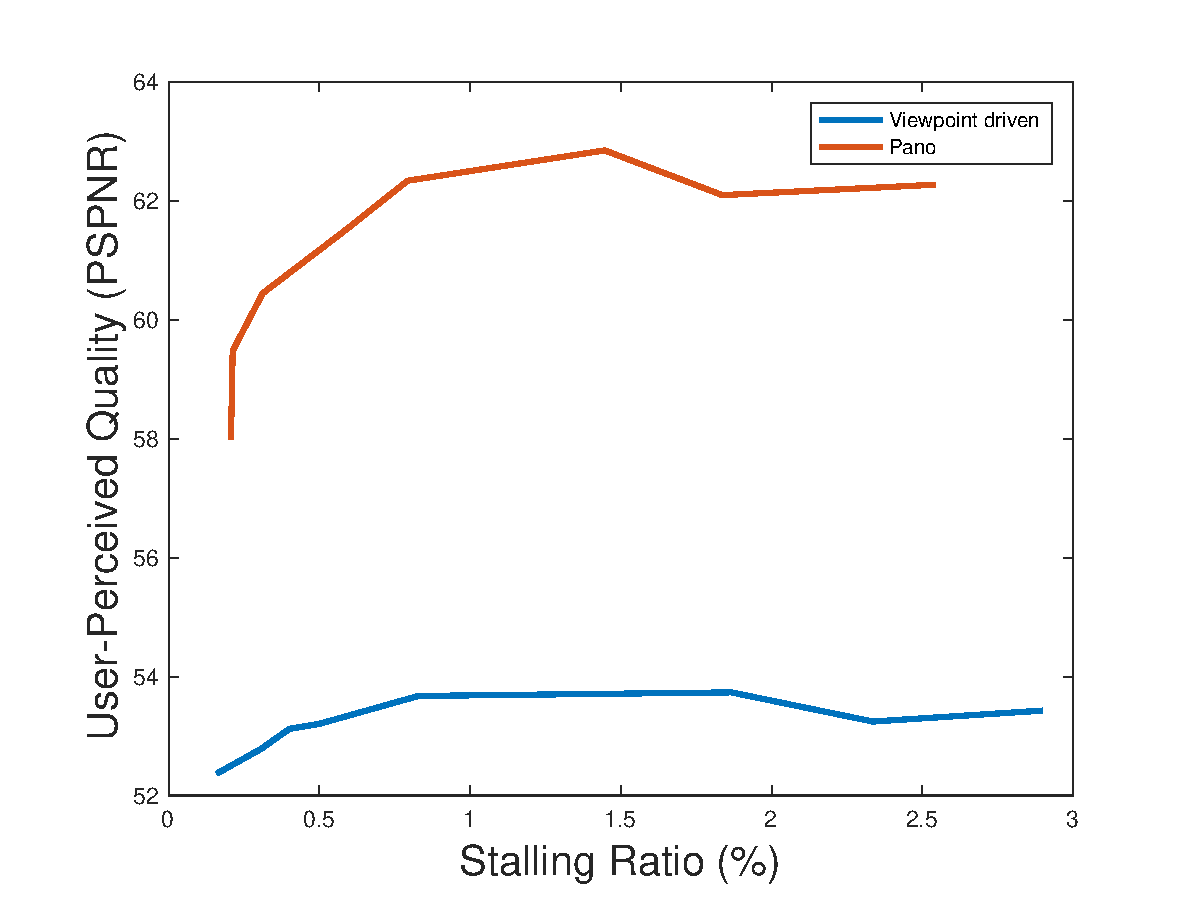
\includegraphics[width=3in]{images/first_image.eps}
  \caption{Performance comparison of Pano v.s. traditional viewpoint-driven video streaming under average throughput of 1Mbps, with bandwidth fluctuation. Each plot indicates a video session. We present 75\% ellipse confidence area.}
  \label{first_image}
  \end{figure}

\textbf{Contributions and Roadmap:}
\begin{itemize}
\item Identifying key visual characteristics which influence user-perceived quality in VR display and estimate potential improvement for it. (\S 2)
\item Identifying key challenges of building a practical perceived-quality-driven VR video streaming system and present our solutions. (\S 3-6)
\item Real-world evaluation that demonstrates substantial performance improvement by PQVRS (\S 7-8).
\end{itemize}
